\documentclass{article}
\usepackage{amsmath}
\usepackage{amssymb}
\usepackage{fancyhdr}
\usepackage[utf8]{inputenc}
\usepackage{tcolorbox}
\usepackage[left=1in, right=1in, top=1.5in, bottom=1in]{geometry}
\usepackage{tikz}
\usepackage{enumerate}
\usepackage{enumitem}
\usepackage{pgfplots}
\pagestyle{fancy}
\fancyhf{} % Clear all header and footer fields
\fancyhead[L]{Your Name} % Left header with name
\fancyhead[R]{September 4th 2025} % Right header with date
\renewcommand{\headrulewidth}{0.4pt} % Horizontal line below the header

\begin{document}

% Main title
\begin{center}
    \Large \textbf{Math 115E Activity 3} \\
    \vspace{0.2cm}
    \normalsize Chapter 2 Section 2 \\
    \normalsize What are functions?
\end{center}
\textbf{Introduction to Intercepts of a graph and how to identify them}

\vspace{1cm} % Add space between the title and the first exercise
\noindent
\begin{minipage}[c]{0.45\textwidth}
    \begin{enumerate}
        
        \item For graph (A) what are the x-intercepts and y-intercepts?
        \vspace{1cm}
        \item For graph (B) what are the x-intercepts and y-intercepts?
        \vspace{1cm}
        \item For graph (C) what are the x-intercepts and y-intercepts?     
        \vspace{1cm}
        \item For graph (D) what are the x-intercepts and y-intercepts?
        \vspace{1cm}
        \item For graph (E) what are the x-intercepts and y-intercepts?
        \vspace{1cm}
        \item For graph (F) what are the x-intercepts and y-intercepts?
        \vspace{1cm}
        \item For graph (G) what are the x-intercepts and y-intercepts?
        \vspace{1cm}
        \item For graph (H) what are the x-intercepts and y-intercepts?
        \vspace{1cm}
        \item For graph (I) what are the x-intercepts and y-intercepts?

    \end{enumerate}
\end{minipage}%
\hfill
\begin{minipage}[c]{0.50\textwidth} % Minipage for the TikZ graph (increased width slightly for labels)
    \centering % Center the TikZ picture within its minipage
    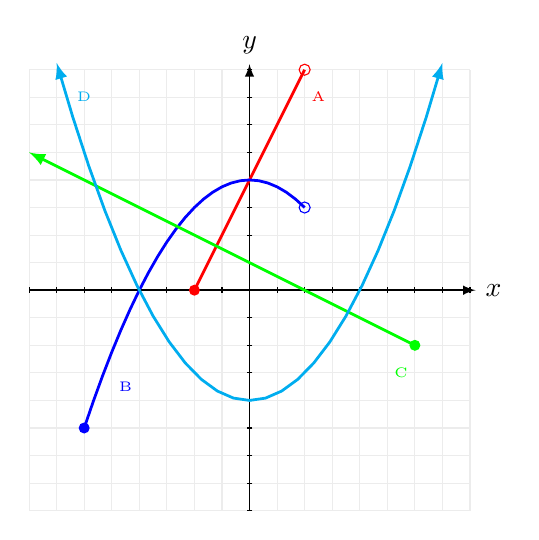
\begin{tikzpicture}[scale=0.35]
        \draw[gray!15,step=1cm] (-8,-8) grid (8,8);
        \draw[line width=0.2mm, -latex] (-8,0) -- (8.2,0) node[right] {$x$};
        % The \foreach loop for x-axis numbers has been modified
        \foreach \x in {-8,...,8} \draw (\x,.1)--(\x,-.1);
        \draw[line width=0.2mm,  -latex] (0,-8) -- (0,8.2) node[above] {$y$};
        % The \foreach loop for y-axis numbers has been modified
        \foreach \y in {-8,...,8} \draw (.1,\y)--(-.1,\y);
        % Red line with adjusted label 'A'
        \draw[red,line width=1pt] plot[domain= -2:2] (\x,{2*\x+4}) node[font=\tiny] at (2.5, 7) {A};
        \fill[red] (-2, 0) circle (0.2);
        \draw[red] (2, 8) circle (0.2);
        % Blue line with adjusted label 'B'
        \draw[blue,line width=1pt] plot[domain= -6:2] (\x,{-0.25*\x*\x+4}) node[font=\tiny] at (-4.5, -3.5) {B};
        \fill[blue] (-6, -5) circle (0.2);
        \draw[blue] (2, 3) circle (0.2);

        % Green line with adjusted label 'C'
        \draw[green,line width=1pt, latex-] plot[domain= -8:6] (\x,{-0.5*\x+1}) node[font=\tiny] at (5.5, -3) {C};
        \fill[green] (6, -2) circle (0.2);
        % Cyan line with adjusted label 'D'
        \draw[cyan,line width=1pt, latex-latex] plot[domain= -7:7] (\x,{0.25*\x*\x-4}) node[font=\tiny] at (-6, 7) {D};    \end{tikzpicture}
    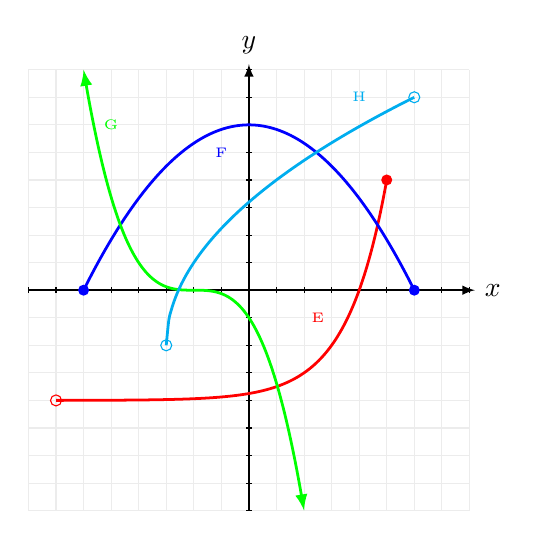
\begin{tikzpicture}[scale=0.35]
        \draw[gray!15,step=1cm] (-8,-8) grid (8,8);
        \draw[line width=0.2mm, -latex] (-8,0) -- (8.2,0) node[right] {$x$};
        % The \foreach loop for x-axis numbers has been modified
        \foreach \x in {-8,...,8} \draw (\x,.1)--(\x,-.1);
        \draw[line width=0.2mm,  -latex] (0,-8) -- (0,8.2) node[above] {$y$};
        % The \foreach loop for y-axis numbers has been modified
        \foreach \y in {-8,...,8} \draw (.1,\y)--(-.1,\y);

        % Red line with adjusted label 'E'
        \draw[red,line width=1pt] plot[smooth, samples=100, domain= -7:5] (\x,{2^(\x-2) - 4}) node[font=\tiny] at (2.5, -1) {E};
        \draw[red] (-7, -4) circle (0.2);
        \fill[red] (5, 4) circle (0.2);
        % Blue line with adjusted label 'F'
        \draw[blue,line width=1pt] plot[smooth, samples=100, domain= -6:6] (\x,{-1/6*(\x-6)*(\x+6)}) node[font=\tiny] at (-1, 5) {F};
        \fill[blue] (-6, 0) circle (0.2);
        \fill[blue] (6, 0) circle (0.2);
        % Green line with adjusted label 'G'
        \draw[green,line width=1pt, latex-latex] plot[smooth, samples=100, domain= -6:2] (\x,{-1/8*(\x+2)^3}) node[font=\tiny] at (-5, 6) {G};
        % Cyan line with adjusted label 'H'
        \draw[cyan,line width=1pt] plot[smooth, samples=100, domain= -3:6] (\x,{3*sqrt(\x+3) - 2}) node[font=\tiny] at (4, 7) {H};
        \draw[cyan] (-3, -2) circle (0.2);
        \draw[cyan] (6, 7) circle (0.2);
    \end{tikzpicture}
    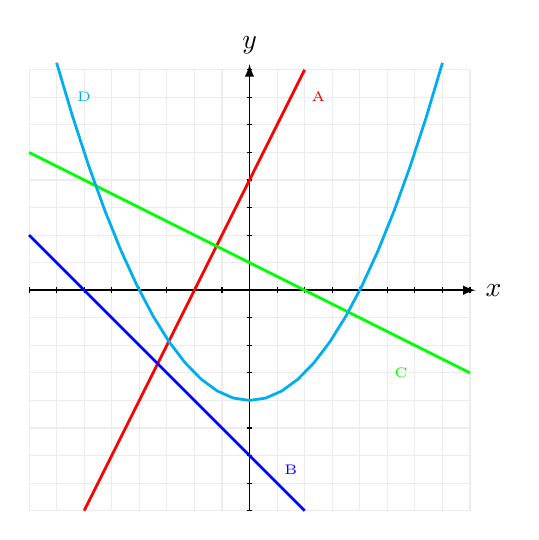
\begin{tikzpicture}[scale=0.35]
        \draw[gray!15,step=1cm] (-8,-8) grid (8,8);
        \draw[line width=0.2mm, -latex] (-8,0) -- (8.2,0) node[right] {$x$};
        % The \foreach loop for x-axis numbers has been modified
        \foreach \x in {-8,...,8} \draw (\x,.1)--(\x,-.1);
        \draw[line width=0.2mm,  -latex] (0,-8) -- (0,8.2) node[above] {$y$};
        % The \foreach loop for y-axis numbers has been modified
        \foreach \y in {-8,...,8} \draw (.1,\y)--(-.1,\y);
        % Red line with adjusted label 'A'
        \draw[red,line width=1pt] plot[domain= -6:2] (\x,{2*\x+4}) node[font=\tiny] at (2.5, 7) {A};

        % Blue line with adjusted label 'B'
        \draw[blue,line width=1pt] plot[domain= -8:2] (\x,{-1*\x-6}) node[font=\tiny] at (1.5, -6.5) {B};

        % Green line with adjusted label 'C'
        \draw[green,line width=1pt] plot[domain= -8:8] (\x,{-0.5*\x+1}) node[font=\tiny] at (5.5, -3) {C};

        % Cyan line with adjusted label 'D'
        \draw[cyan,line width=1pt] plot[domain= -7:7] (\x,{0.25*\x*\x-4}) node[font=\tiny] at (-6, 7) {D};
    \end{tikzpicture}
\end{minipage}

\end{document}